
\newcommand{\bbbar}{\ensuremath{\text{b}\overline{\text{b}}}\xspace}
\newcommand{\ttbar}{\ensuremath{\text{t}\overline{\text{t}}}\xspace}
\newcommand{\ttH}{\ensuremath{\ttbar\text{H}}\xspace}
\newcommand{\tH}{\ensuremath{\text{tH}}\xspace}
\newcommand{\Hbb}{\ensuremath{\text{H}\rightarrow\bbbar}\xspace}
\newcommand{\ttHF}{\ensuremath{\ttbar+\text{HF}}\xspace}
\newcommand{\TeV}{\ensuremath{\,\text{Te\hspace{-.08em}V}}\xspace}
\providecommand{\fbinv}{\mbox{\ensuremath{\,\text{fb}^\text{$-$1}}}\xspace}
\newcommand{\tth}{\ensuremath{\Pqt\Pqt\PH}\xspace}
\newcommand{\ww}{\ensuremath{\PW\PW}\xspace}
\newcommand{\hww}{\ensuremath{\PH\to\ww}\xspace}
\newcommand{\tautau}{\ensuremath{\Pgt\Pgt}\xspace}
\newcommand{\tHW}{\ensuremath{\Pqt\PH\PW}\xspace}
\newcommand{\tHq}{\ensuremath{\Pqt\PH\PQq}\xspace}
\newcommand{\zz}{\ensuremath{\PZ\PZ}\xspace}
\newcommand{\bb}{\ensuremath{\PQb\PQb}\xspace}
\newcommand{\hbb}{\ensuremath{\PH\to\bb}\xspace}
\renewcommand{\gg}{\ensuremath{\PGg\PGg}\xspace}
\newcommand{\hgg}{\ensuremath{\PH\to\gg}\xspace}
\providecommand{\ttjets}{\ensuremath{\PQt\PQt\text{+}\text{jets}}\xspace}

\subsubsection{Measurements in \ttH and \tH production modes}
\begin{center}{\it by A. Calandri, M. Schr\"oder} \end{center}

%\author{Alessandro Calandri, Matthias Schr\"oder}
%\date{July 31th, 2018}

One of the main targets of the High-Luminosity LHC (HL-LHC) upgrade is to achieve precision measurements of the Higgs boson properties. The Yukawa coupling of the Higgs boson to the top quark is expected to be of the order of unity and could be partially sensitive to effects beyond the Standard Model (SM). Therefore, a direct measurement of the coupling of the Higgs boson to top quarks is extremely important to access possible deviations in the top quark's Yukawa couplings due to couplings to new particles. Such a measurement can be performed by measuring the rate of the process where the Higgs boson is produced in association with a pair of top quarks (\ttH) or a single top quark (\tH). Even though the \ttH process is characterized by a small cross section compared to the dominant gluon fusion Higgs boson production (approximately two orders of magnitude smaller), the signature with top quarks in the final state can be exploited to reconstruct the event and gives access to many Higgs boson decay modes.
The SM \tH production cross-section is yet smaller by a factor five, but due to interference effects between diagrams with top-Higgs and W-boson-Higgs couplings, the process allows access to the sign of the top-Higgs Yukawa coupling.
The ATLAS and CMS Collaborations have searched for the \ttH and \tH production with LHC Run 2 data of 2015, 2016, and 2017, and observed the Higgs boson production in association with a top-quark pair \cite{Aaboud:2018urx,Sirunyan:2018hoz}. The analyses are sensitive to a large variety of final-state event topologies, H$\rightarrow$WW$^{*}$, H$\rightarrow$ZZ$^{*}$, H$\rightarrow \tau^{+}\tau^{-}$, H$\rightarrow b\bar{b}$ and H$\rightarrow \gamma\gamma$. They are all considered in the analyses and in the coupling combination.  

One of the main goal of the HL-LHC upgrade is to allow precision measurements of the Higgs boson properties, especially for what regards the Yukawa coupling of the Higgs boson to top quarks. The projection studies performed by ATLAS and CMS and reported in this Section are based on the extrapolation of Run 2 results to the 3000 fb$^{-1}$ integrated luminosity expected at HL-LHC. In addition, the signal and background production cross sections are scaled to account for the increase of the LHC center-of-mass energy expected for HL-LHC ($\sqrt{s}$=13 TeV $\rightarrow$ 14 TeV).

The Run 2 extrapolation to 3000 fb$^{-1}$ will provide much better precision than previously expected. As a consequence, the limitation induced by the current knowledge of the systematics uncertainty will occur at a lower integrated luminosity than what has been previously expected if the magnitude of such uncertainties are not reduced.
For example, the studies by the ATLAS Collaboration reported in \cite{ATL-PHYS-PUB-2018-010} focus on the most critical theory uncertainties in \ttH (H decaying to multileptons, ML, i.e.  H$\rightarrow$WW$^{*}$, H$\rightarrow$ZZ$^{*}$, H$\rightarrow \tau^{+}\tau^{-}$ and H$\rightarrow \gamma\gamma$) and their impact on the cross section and signal strength measurements with 3000 fb$^{-1}$, while the studies by CMS Collaboration reported in \cite{CMS-PAS-FTR-18-011} investigate \ttH production in the \Hbb final state as well as \tH production in the ML final state.
Figure \ref{fig:topyukawa:theoATLAS} (a) shows the breakdown of uncertainties on the signal strength ($\mu$) for the ttH ML channel as a function of the integrated luminosity. These uncertainties affect the signal strength and not the cross section measurement accuracy. The main source of signal theory uncertainty for the measurement is the parton shower modeling which is evaluated from the comparison of alternative simulated samples as in the Run 2 measurement \cite{Aaboud:2017jvq}. It is the main component of the '\ttH model (acceptance)' label in Figure \ref{fig:topyukawa:theoATLAS} (a) and it becomes dominant over the statistical precision ('data statistics') above 300 fb$^{-1}$. In addition, the background modeling and the experimental systematics are highly ranked in the measurement but they are expected to reduce significantly at HL-LHC. Similar conclusions can be drawn in the \ttH, H$\rightarrow \gamma\gamma$ final state as shown in Figure \ref{fig:topyukawa:theoATLAS} (b). In this case, the '\ttH model (acceptance)' systematic uncertainty matches the statistical accuracy of the measurement for the full HL-LHC dataset (3000 fb$^{-1}$). 
In the \Hbb channel, the sensitivity of the Run 2 analysis is limited by the modelling of the \ttbar + heavy-flavour jets (\ttHF) background Figure \ref{fig:topyukawa:theoATLAS} (c).
Substantial improvement in analysis precision is expected to arise from direct measurements of the \ttHF cross-sections, exploiting the large amount of data at the HL-LHC and the capability of the fit to constrain these uncertainties.
\begin{figure}[!htbp]
  \begin{center}
    \subfloat[]{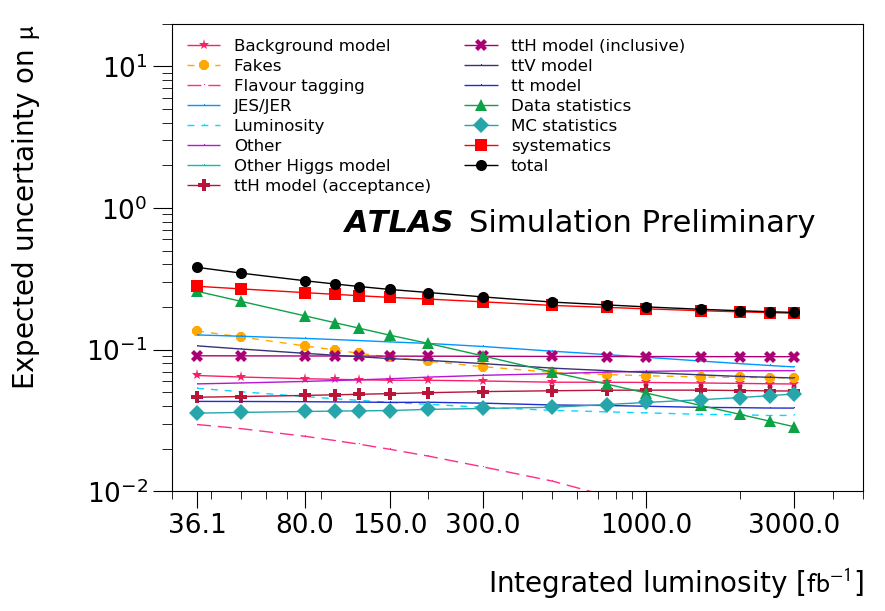
\includegraphics[width=0.34\textwidth]{section2/plots/breakdown_ML.png}}
    \subfloat[]{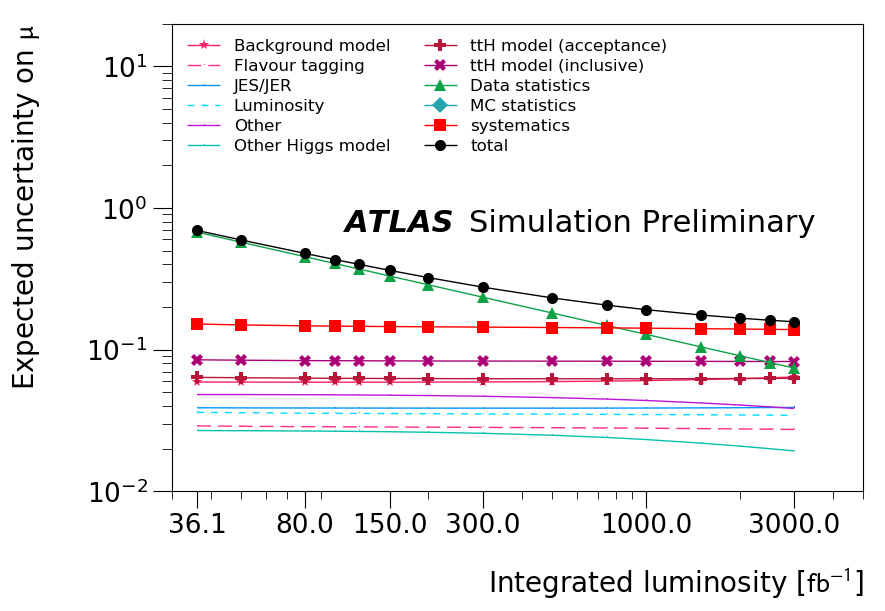
\includegraphics[width=0.34\textwidth]{section2/plots/breakdown_gg.png}}
    % \subfloat[]{\includegraphics[width=0.34\textwidth]{section2/plots/breakdown_bb.png}}
    \textbf{Add plot: CMS ttH bb}
    \caption{Breakdown of uncertainties affecting the Higgs boson signal strength for the \ttH multileptons (a), \ttH, H$\rightarrow\gamma\gamma$ (b), and \ttH, \Hbb (c) channels as a function of the integrated luminosity for $\sqrt{s}$=14 TeV.}
    \label{fig:topyukawa:theoATLAS}
  \end{center}
\end{figure}


\subsubsubsection{Results on top-Yukawa coupling extrapolations at HL-LHC in ATLAS and CMS}
As reported earlier in this Section, the extrapolation is based on the scaling of the current Run 2 analyses performed by the ATLAS and CMS experiments to HL-LHC conditions ($\int \mathcal{L}dt$=3000 fb$^{-1}$, $\sqrt{s}$=14 TeV).
Two different assumptions about the evolution of the uncertainties are made to reflect a realistic range of the expected result:
they are kept the same as in the Run 2 studies (scenario 1) or the theory uncertainties are halved and th experimental uncertainties are scaled down by the square root of the integrated luminosity until they reach a defined lower limit based on the estimated performance of the upgraded detectors (scenario 2).
Figure \ref{fig} shows the expected precision for ATLAS and CMS on the signal strength ($\Delta\mu$/$\mu$) and on the measured cross section.
This process should be measured with an ultimate uncertainty on the signal strength of approximately AA\% in H$\rightarrow\gamma\gamma$, BB\% (for \ttH) and BBB\% (for \tH) in the multilepton final state, and CC\% in \Hbb. This will provide stringent constraints on possible beyond SM contributions to \ttH. Table \ref{} shows the uncertainty on the Higgs boson signal strength and its breakdown in the statistical component as well as the components from the theory and the experimental systematic uncertainties.
The significance of the \ttH process in the H$\rightarrow \gamma\gamma$, ML, and \bbbar final states is D$\sigma$, E$\sigma$, and F$\sigma$, respectively, while G$\sigma$ are obtained for the \TH process in the ML final state.

\subsubsubsection{Sensitivity to \tH production}

The sensitivity to the $\tH$ process at the HL-LHC is determined by extrapolating a combination of Run~2 analyses based on $35.9\fbinv$ of data at $\sqrt{s}= 13 \TeV$~\cite{CMS-PAS-HIG-18-009}. Two of these  analyses are dedicated searches for $\tHq$: one targets a multi-lepton final state~\cite{CMS-PAS-HIG-17-005} in which the Higgs boson decays to $\ww$, $\zz$ or $\tautau$ pairs, and the other targets the $\hbb$ decay~\cite{CMS_PAS_HIG_17-016}. In both analyses the presence of at least one central b tagged jet and an isolated lepton from the top quark decay is required. Furthermore, the presence of a light quark jet at high pseudorapidity, a unique feature of the $\tHq$ production mode, is exploited. Both analyses also rely heavily on multivariate techniques to discriminate the signal against the large $\ttjets$ background. The $\gg$ final state is also utilised, via a reinterpretation of the inclusive $\hgg$ analysis~\cite{Sirunyan:2018ouh}. In this analysis the $\mathrm{tHq}$ and $\mathrm{tHW}$ processes primarily contribute to the``$\mathrm{t\bar{t}H}$ leptonic'' and ``$\mathrm{t\bar{t}H}$ hadronic'' event categories, and these are included in the combination.


In Figure~\ref{fig:limit} the variation of the expected upper limits on $\mu_{\tH}$ is shown as a function of the integrated luminosity for the S1 and S2 scenarios. The limits are determined assuming a background-only hypothesis in which the $\tth$ process is considered as following the SM epectation ($\mu_{\tth} = 1$). In order to minimize further assumptions on the rate of $\tth$ production, $\mu_{\tth}$ is treated as a free parameter in the fit.
In the S1 scenario the expected median upper limit on $\mu_{\tH}$ at 3000 \fbinv is determined to be 2.35.
The corresponding value in S2 is 1.51. With the $3000 \fbinv$ dataset and foreseen reduction in systematic uncertainties in S2, the expected upper limit on $\mu_{\tH}$ improves by about a factor of eight with respect to the current exclusion.

\begin{figure}[hbtp]
\begin{center}
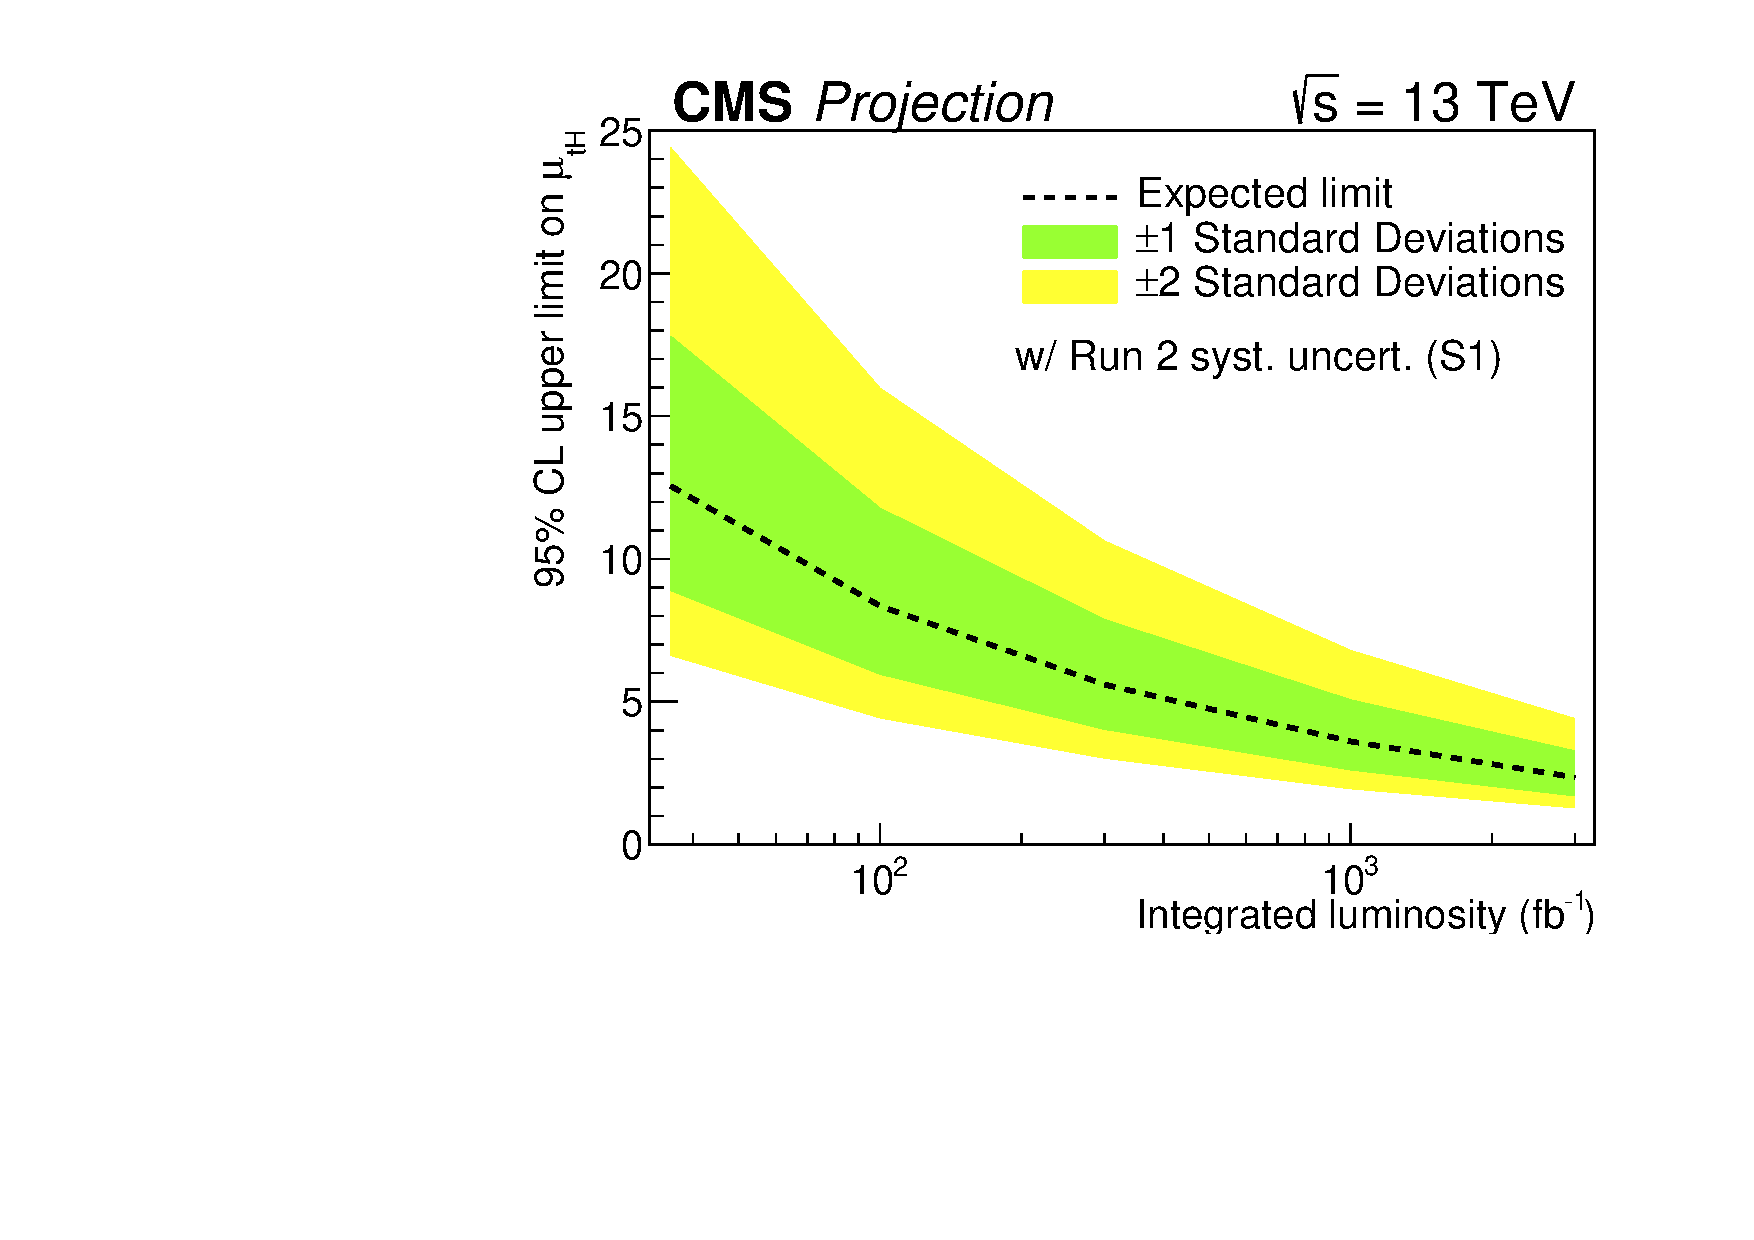
\includegraphics[width=0.45\textwidth]{\main/section2/plots/channels/limits_S1.pdf} \hspace{1cm}
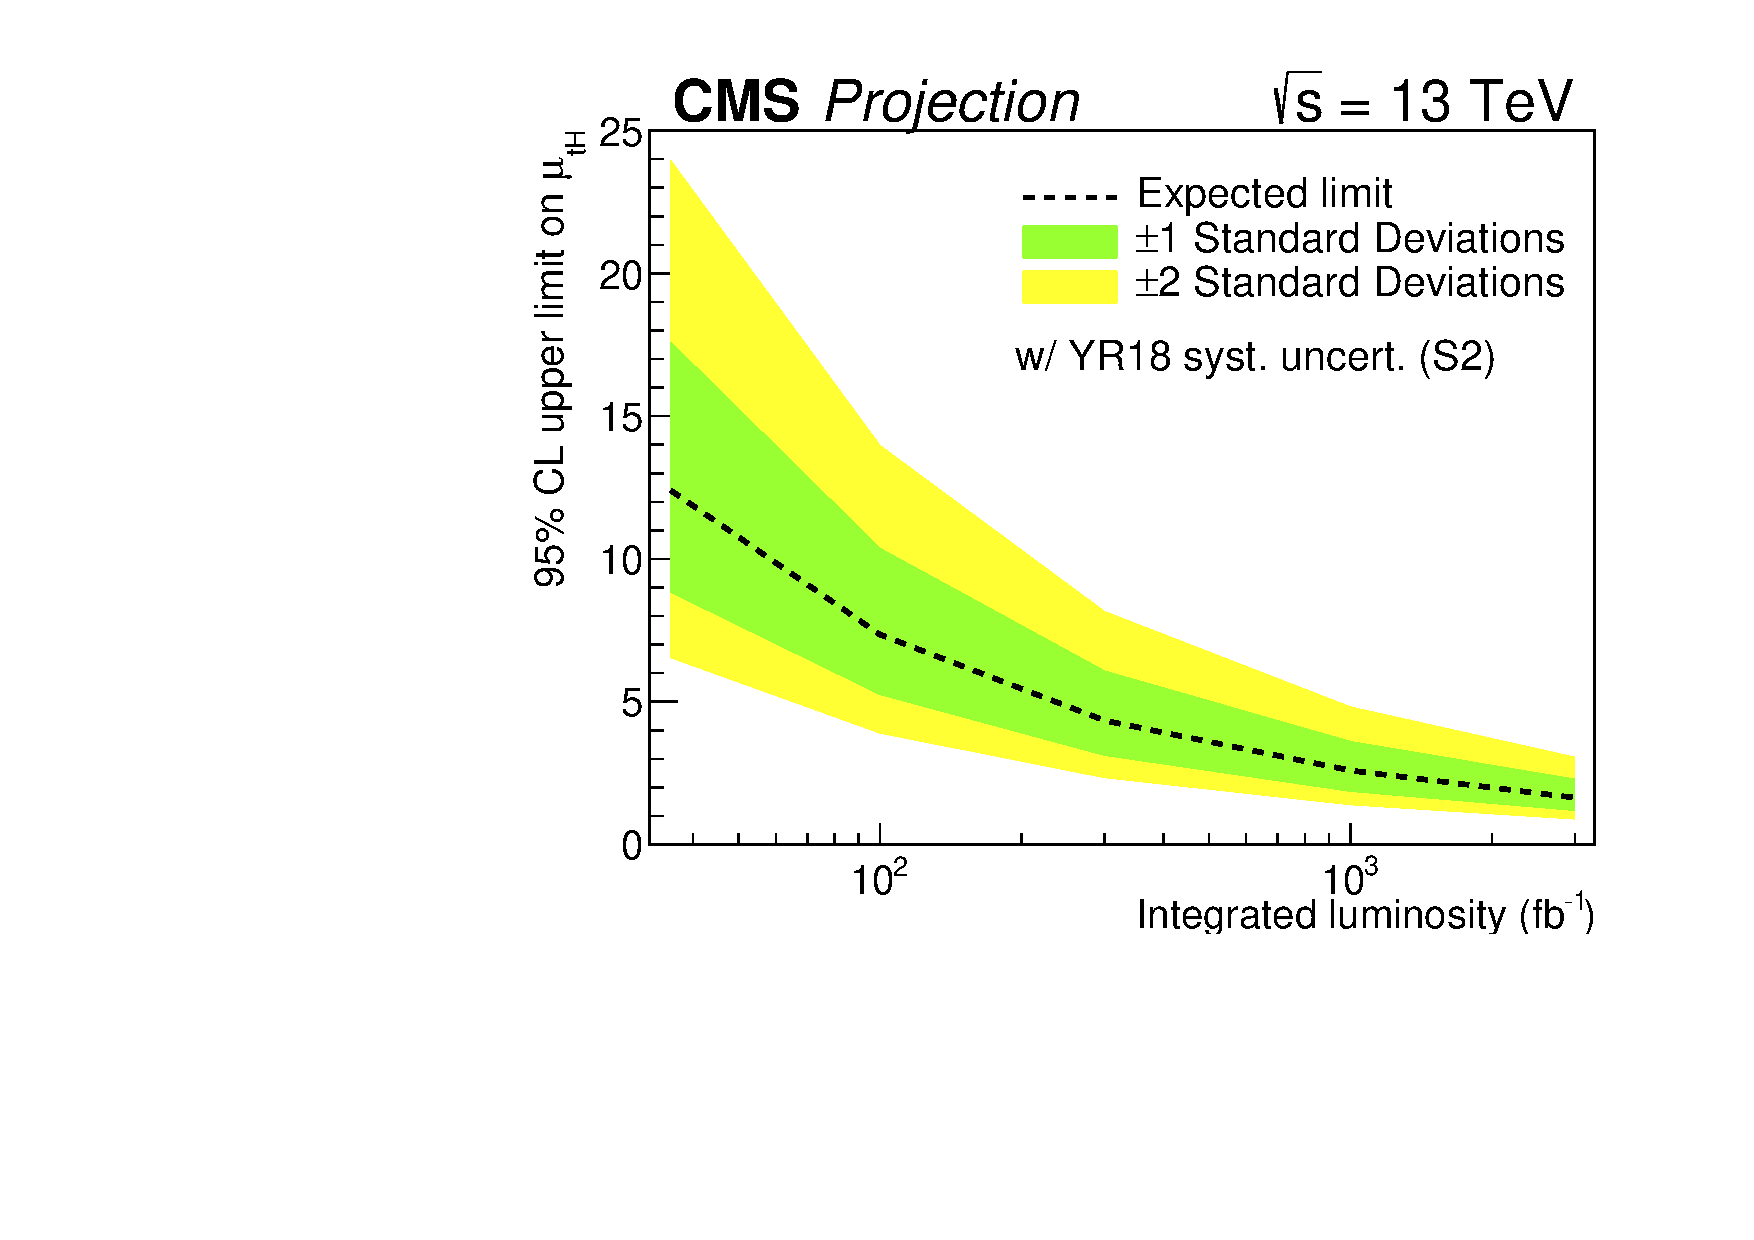
\includegraphics[width=0.45\textwidth]{\main/section2/plots/channels/limits_S2.pdf}
\end{center}
\caption{The variation of expected upper limit on $\mu_{\tH}$ with integrated luminosity for two projection scenarios S1 (with Run~2 systematic uncertainties~\cite{CMS-PAS-HIG-18-009}) and S2 (with YR18 systematic uncertainties).}
\label{fig:limit}
\end{figure}

The evolution of the expected uncertainty on the measurement of $\mu_{\tH}$, assuming the SM rate, is given in Table~\ref{tab:muunc}. Values are given for two cases of background: one in which $\mu_{\tth}$ is unconstrained in the fit, and one in which it is fixed to the SM value of 1. In the latter case the uncertainties are reduced by around $10\%$ at $3000\fbinv$, indicating that a precise simultaneous measurement of the $\tth$ signal strength will be needed to obtain the optimal sensitivity to the $\tH$ channel. In both cases it is found that the reduced systematic uncertainties in S2 improve the precision by up to $30\%$.

\begin{table}[htbp]
\centering
\caption{The $\pm1\sigma$ uncertainties on expected $\mu_{\tH}$=1 for scenarios S1 (with Run~2 systematic uncertainties~\cite{CMS-PAS-HIG-18-009}) and S2 (with YR18 systematic uncertainties) at all three luminosities, considering also the case when $\mu_{\ttH}$ is fixed at the SM value 1.} \label{tab:muunc}
\begin{tabular}{@{} l c c@{\hskip 0.15in} c c }
 \hline
  &  & $\mu_{\tth}$ floating & $\mu_{\tth}$ fixed \\
  \hline
\multirow{3}{*}{S1} & 35.9 \fbinv  & ${}_{-5.8}^{+6.2}$ & ${}_{-5.4}^{+5.8}$ \\[1pt]
                        & 300 \fbinv & ${}_{-2.8}^{+2.9}$ & ${}_{-2.4}^{+2.5}$ \\[1pt]
                        & 3000 \fbinv & ${}_{-1.2}^{+1.2}$ & ${}_{-1.0}^{+1.1}$ \\[4pt]
\hline
\multirow{3}{*}{S2}  & 35.9 \fbinv  & ${}_{-5.8}^{+6.2}$ & ${}_{-5.3}^{+5.8}$ \\[1pt]
                        & 300 \fbinv & ${}_{-2.2}^{+2.2}$ & ${}_{-2.0}^{+2.0}$ \\[1pt]
                        & 3000 \fbinv & ${}_{-0.9}^{+0.9}$ & ${}_{-0.8}^{+0.8}$ \\[4pt]
 \hline
\end{tabular}
\end{table}

\subsubsection{Constraints from differential measurements}
\begin{center}{\it To be written by: T. Klijnsma} \end{center}
